\documentclass[10pt]{article}
\usepackage{graphicx}
\usepackage{pdfpages}
\usepackage{polyglossia}
\usepackage{libertine}
\usepackage[papersize={3.6in,4.8in},hmargin=0.45in, vmargin={0.2in,0.4in}]{geometry}
\usepackage{fancyhdr}
%\usepackage[papersize={3.6in,4.8in},hmargin=0.1in,vmargin={0.1in,0.1in}]{geometry}

\setmainlanguage{english}
\setotherlanguage{arabic}

\newfontfamily\arabicfont[
  Script=Arabic,%
  Numbers=Proportional,%
  Scale=1.5,%
  Ligatures=TeX,
  Mapping=arabicdigits
]{Scheherazade}

\setlength{\footskip}{0pt}

\begin{document}
\pagestyle{fancy}

%%%%%%%%%%%%% Fancy HDR
\lhead{}\chead{}\rhead{}

\lfoot{}
\cfoot{\textarabic{\thepage}}
\rfoot{}

\renewcommand{\headrulewidth}{0.4pt}
\renewcommand{\footrulewidth}{0pt}
%%%%%%%%%%%%

\begin{center}
\rfoot{\small{al-Fātiḥah}}
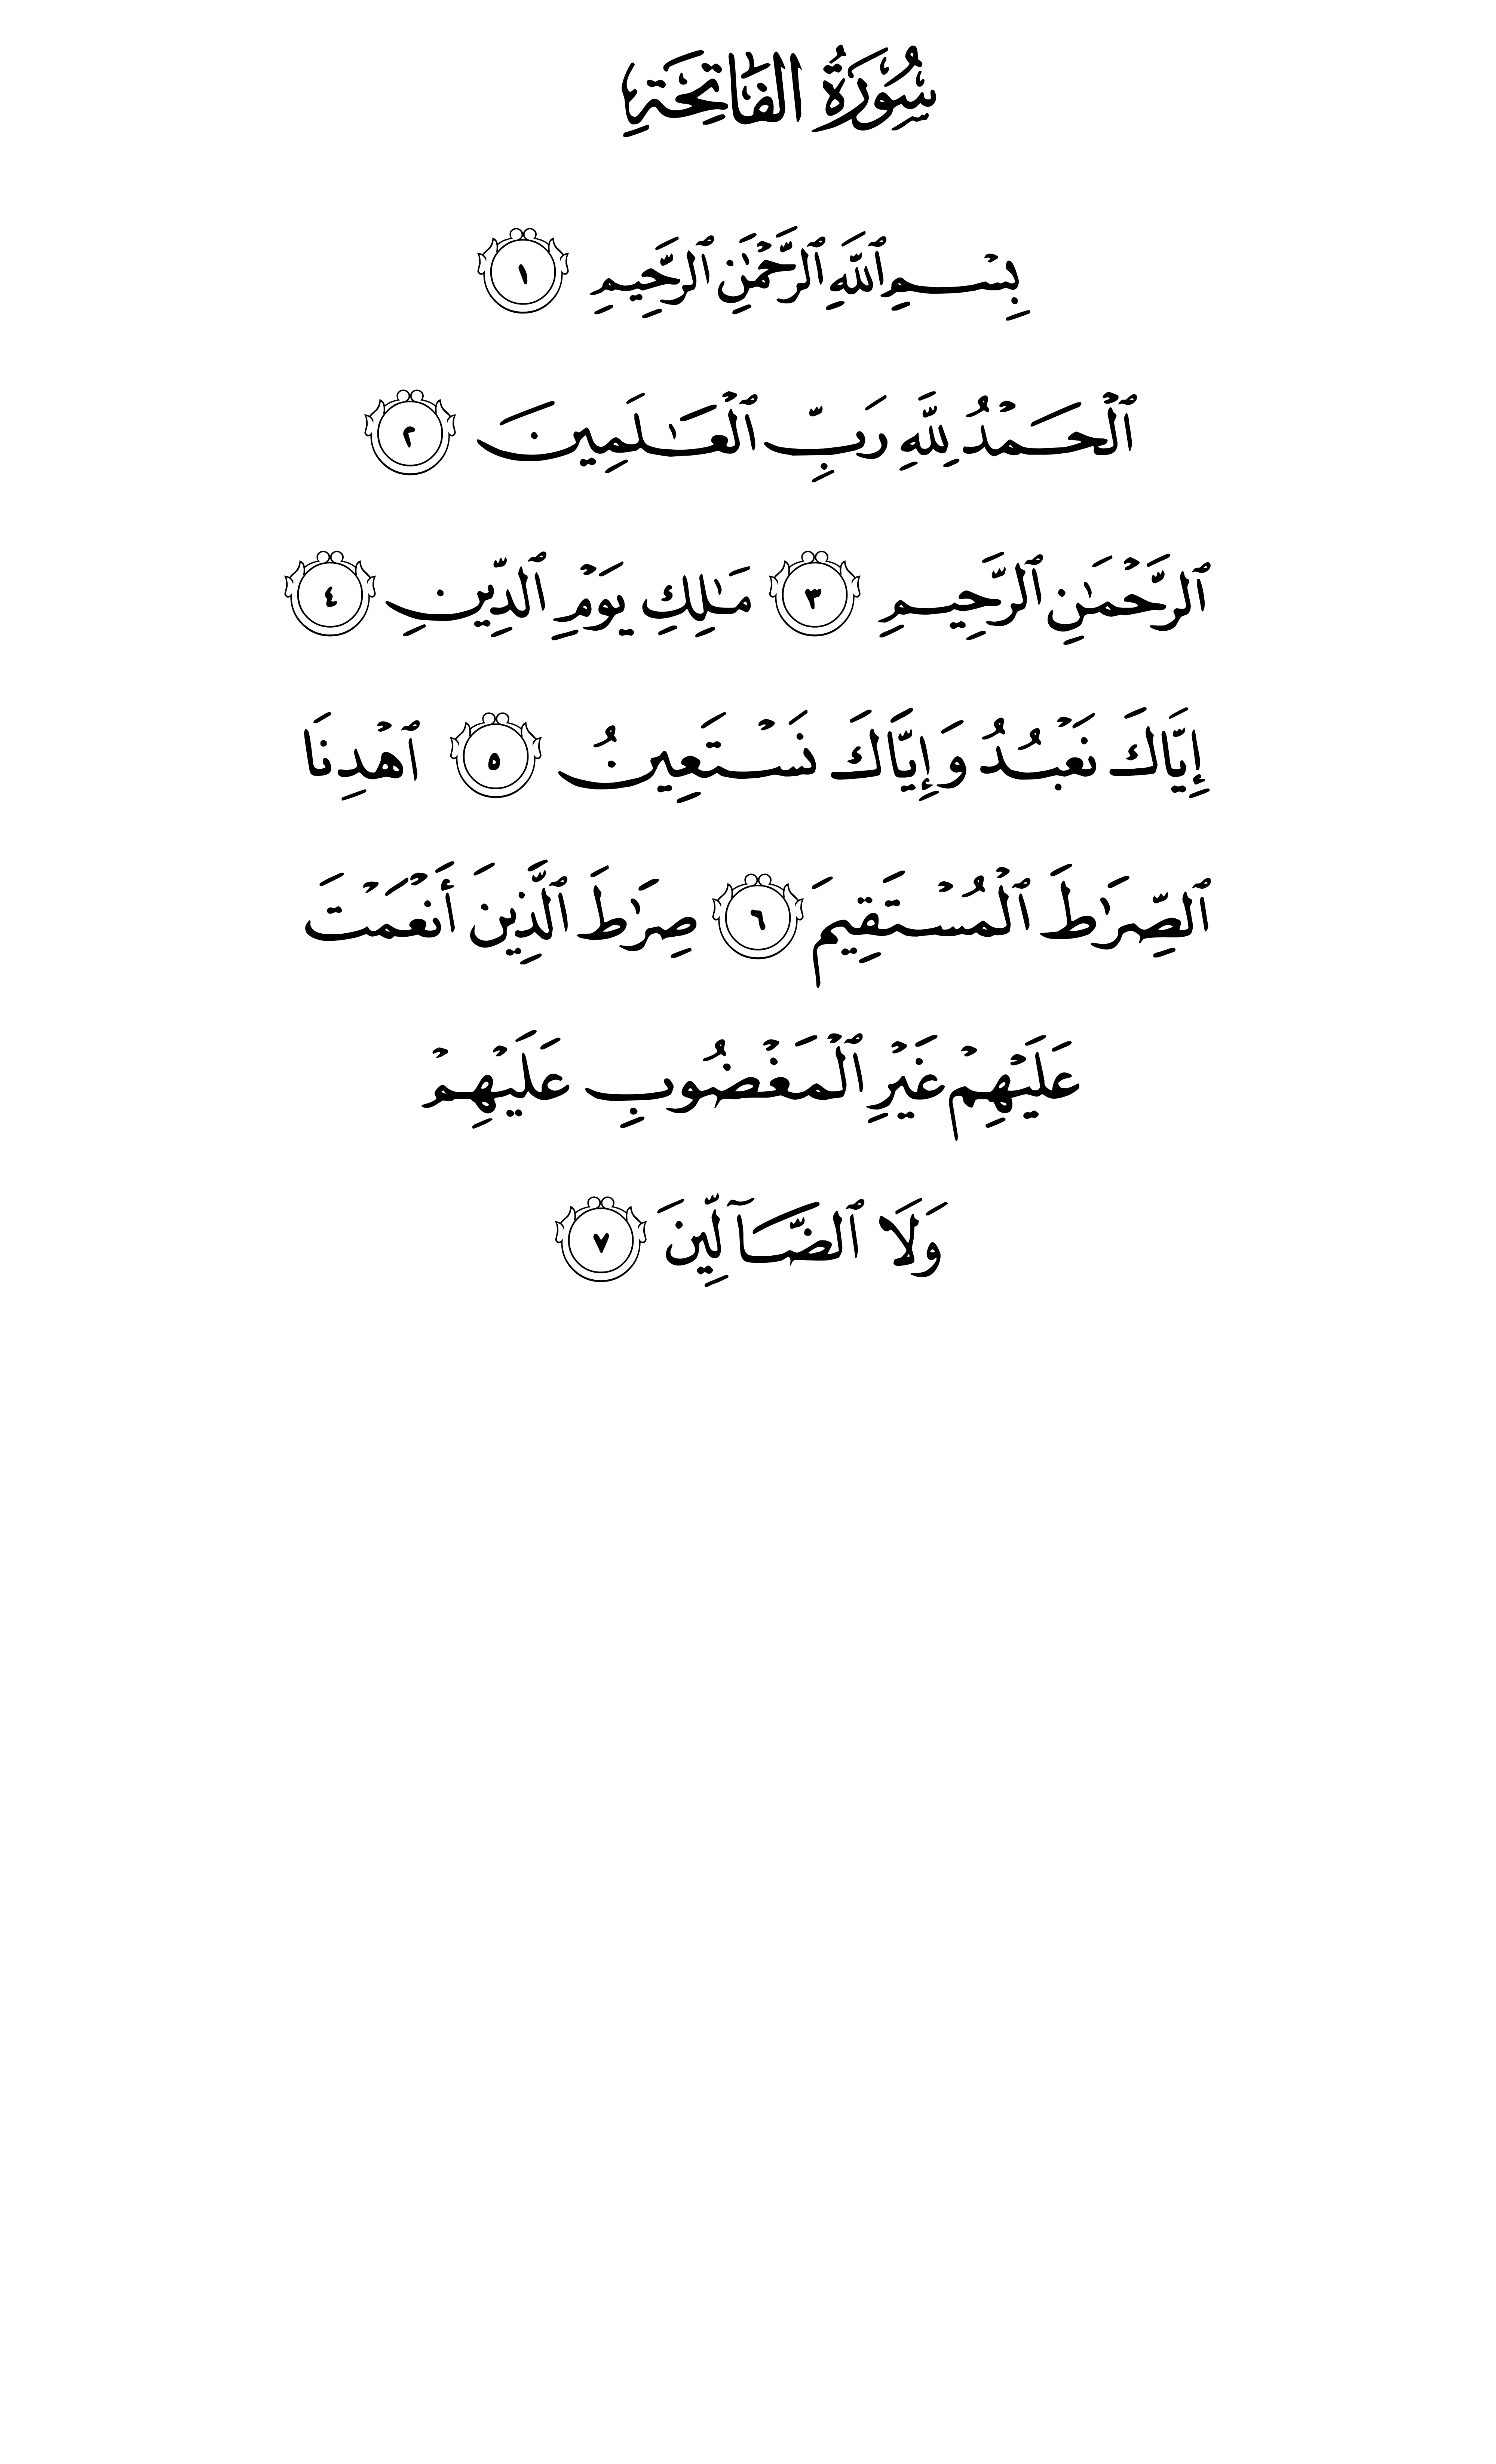
\includegraphics[width=\textwidth,height=\textheight,keepaspectratio]{images/001.png}\newpage
\rfoot{\small{al-Baqarah}}
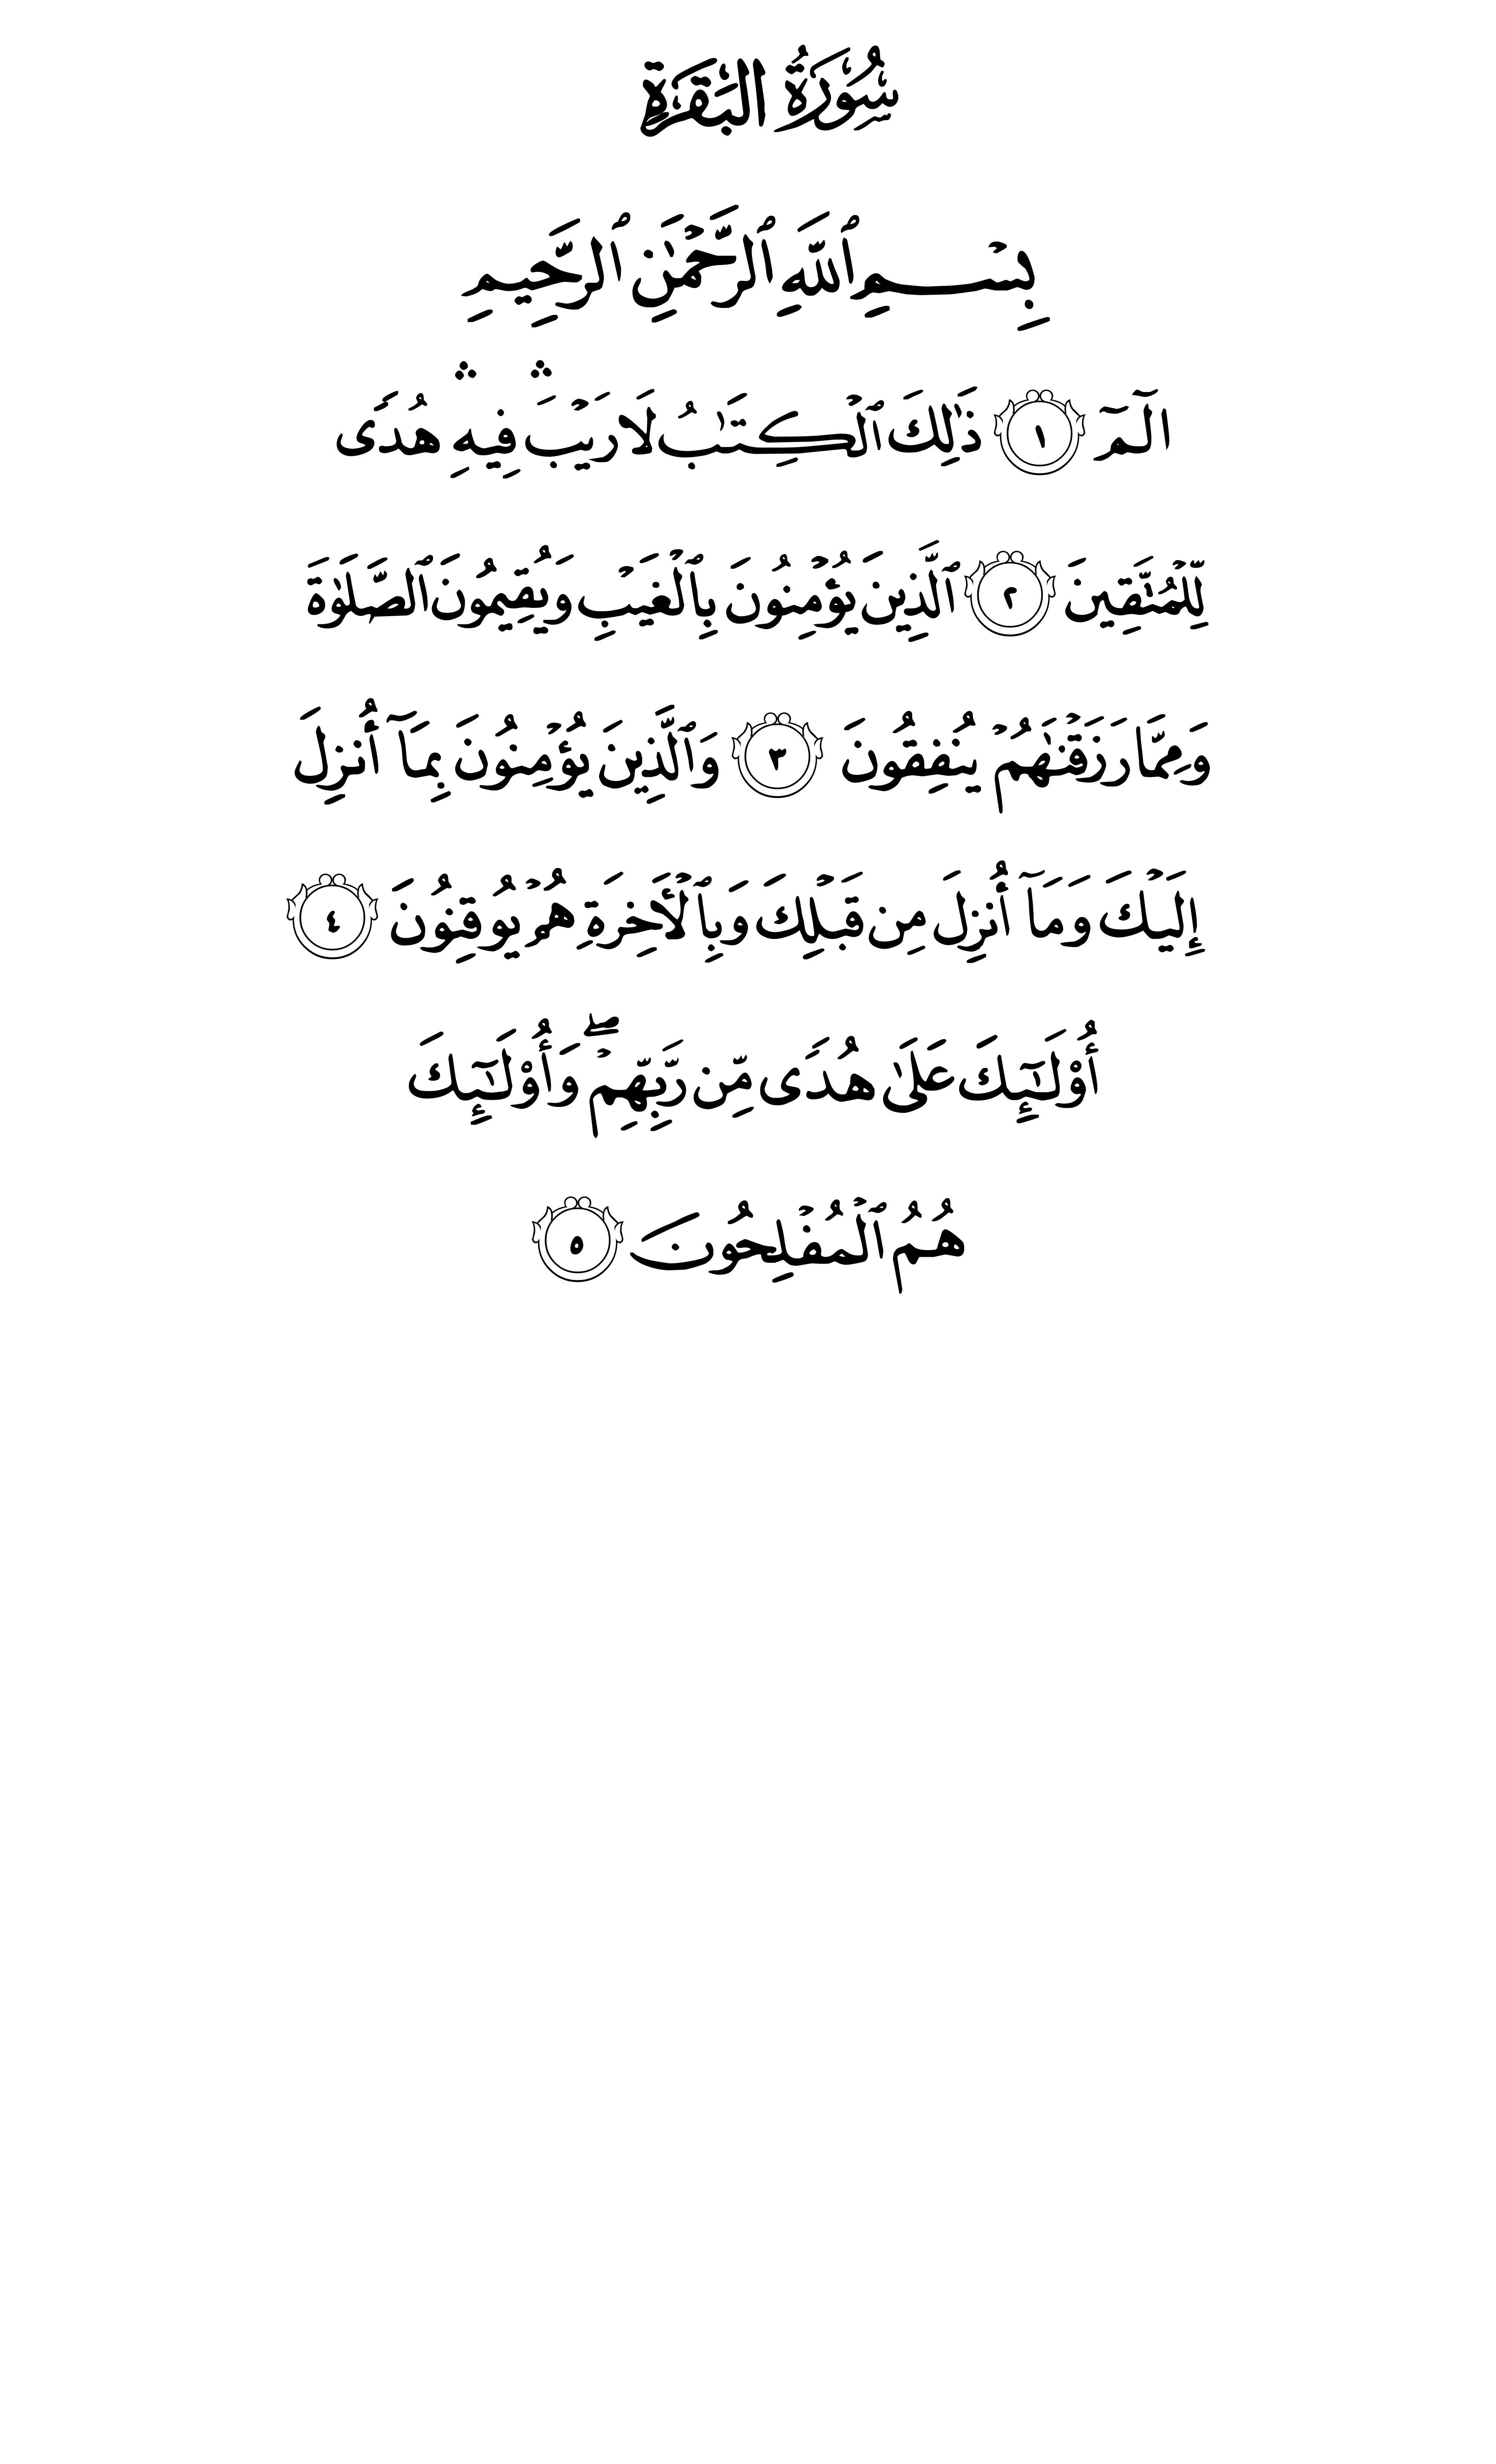
\includegraphics[width=\textwidth,height=\textheight,keepaspectratio]{images/002.png}\newpage
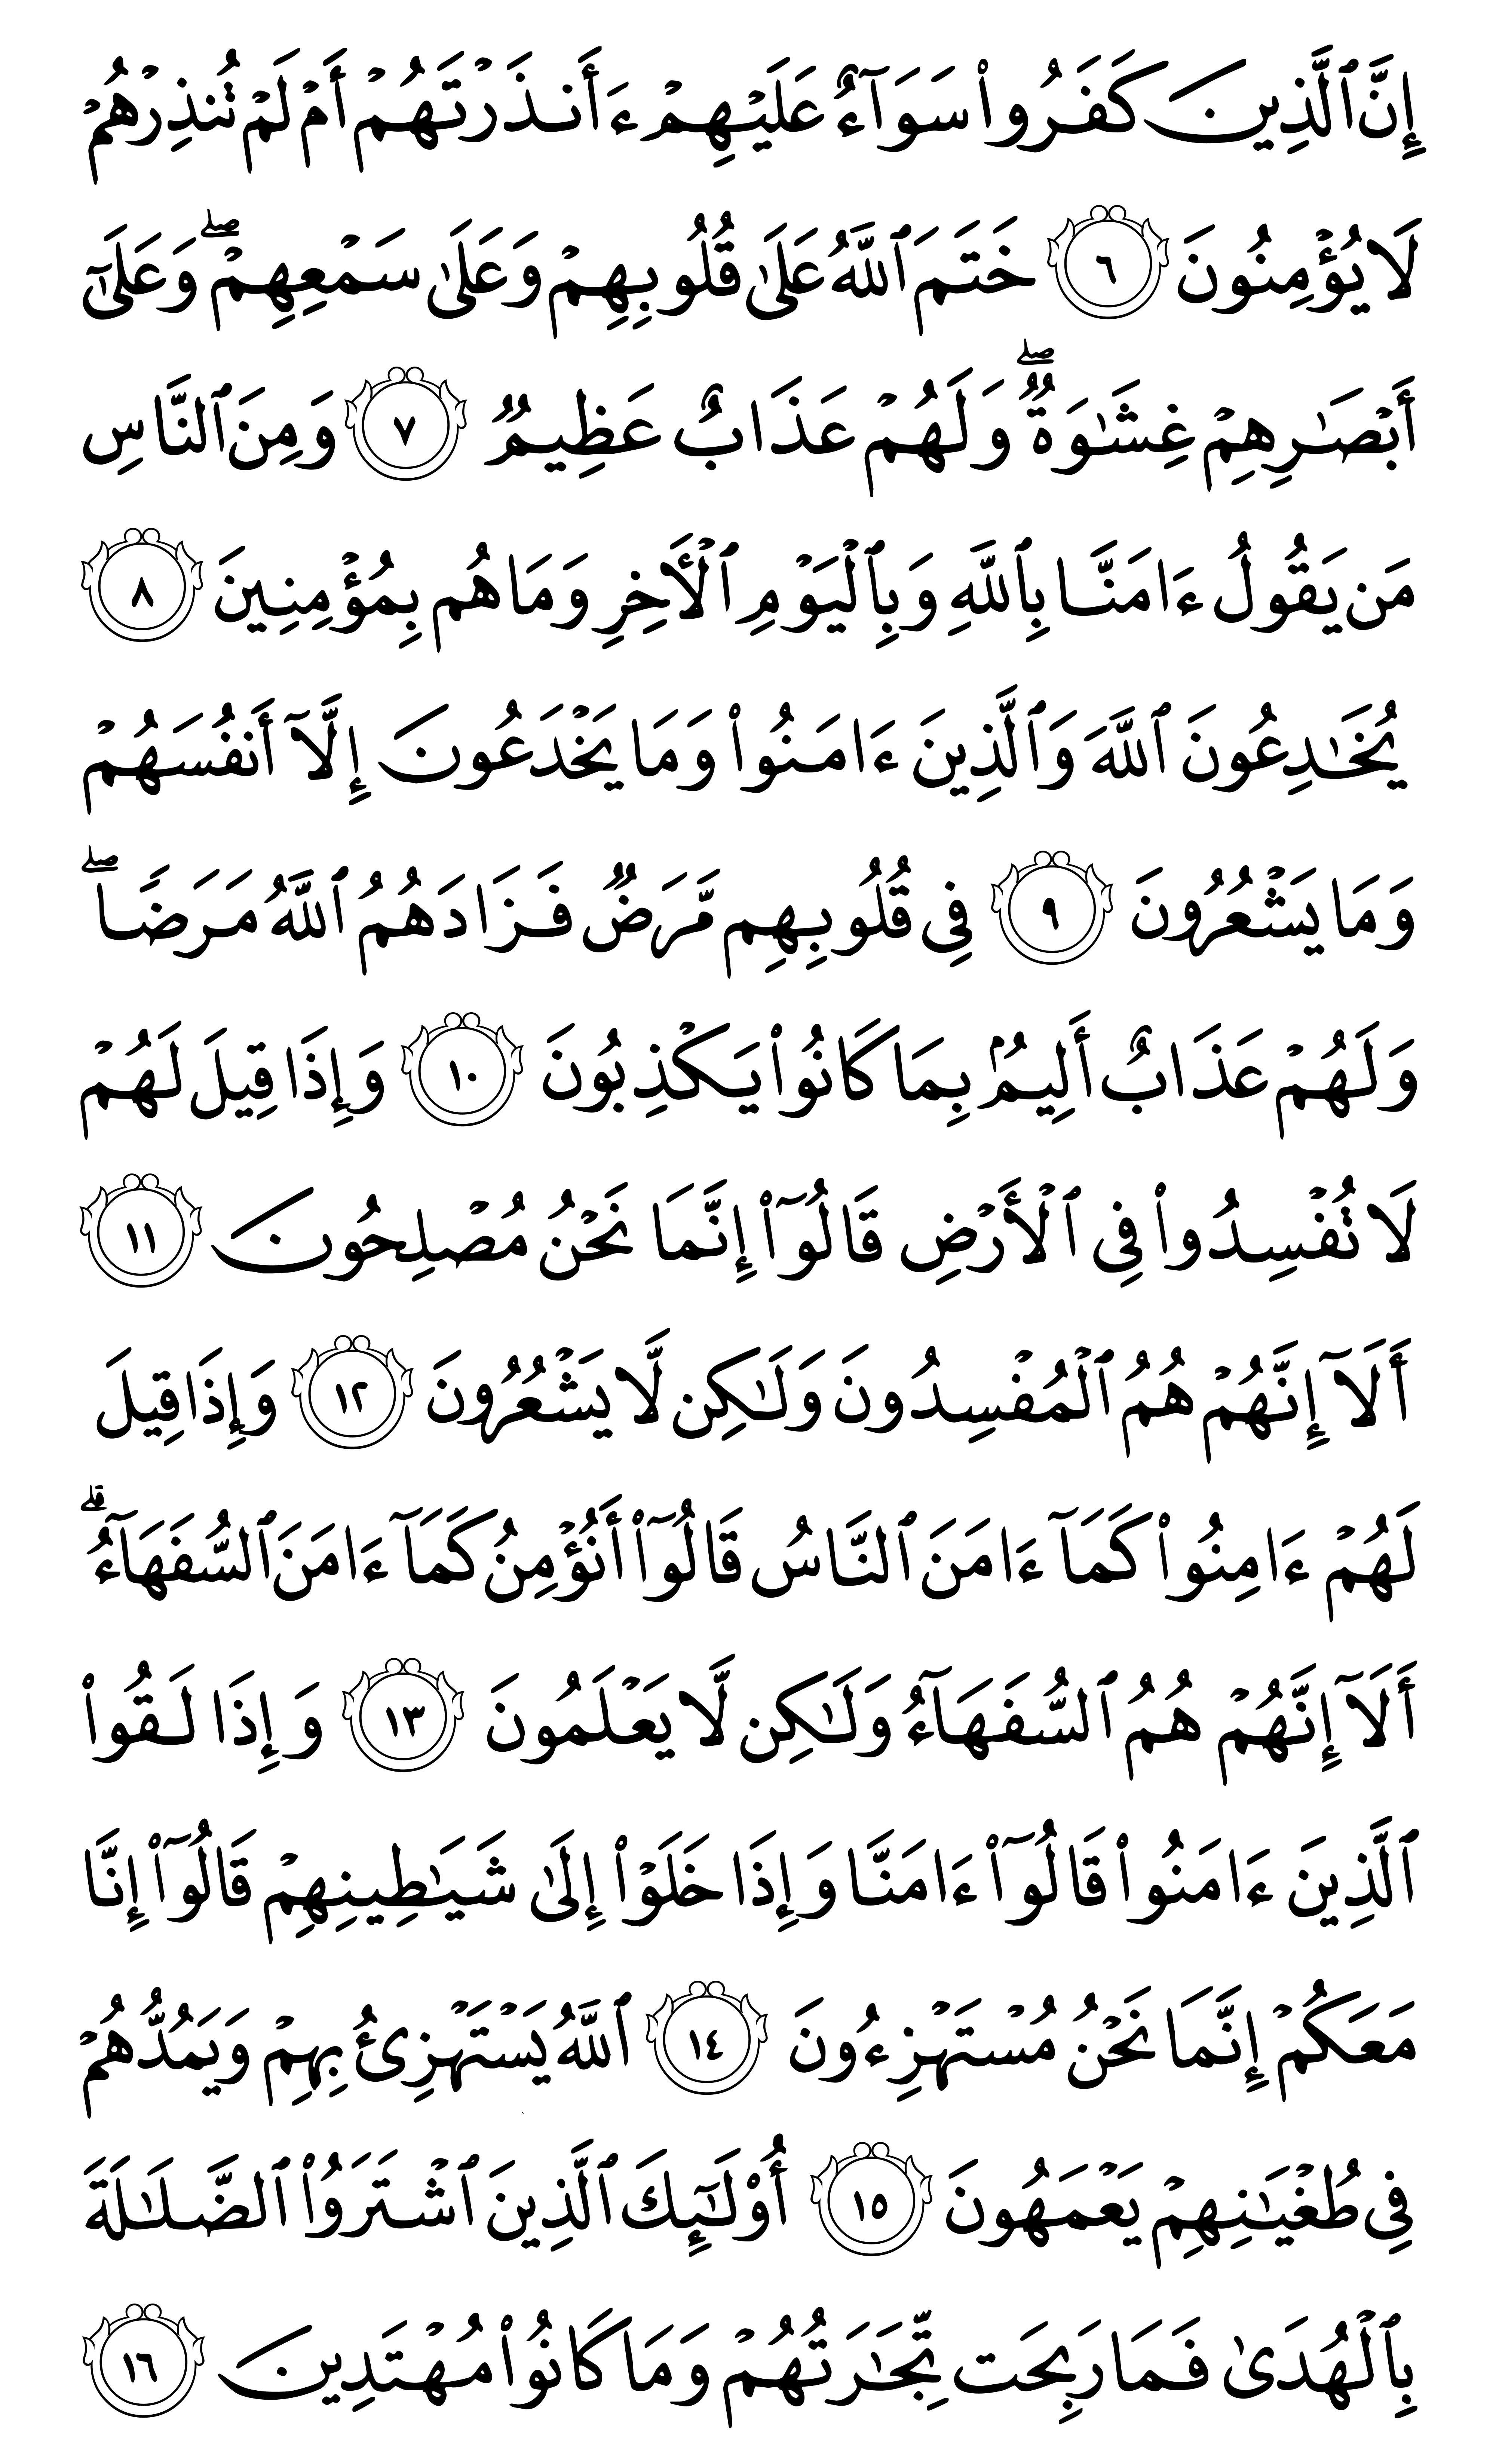
\includegraphics[width=\textwidth,height=\textheight,keepaspectratio]{images/003.png}\newpage
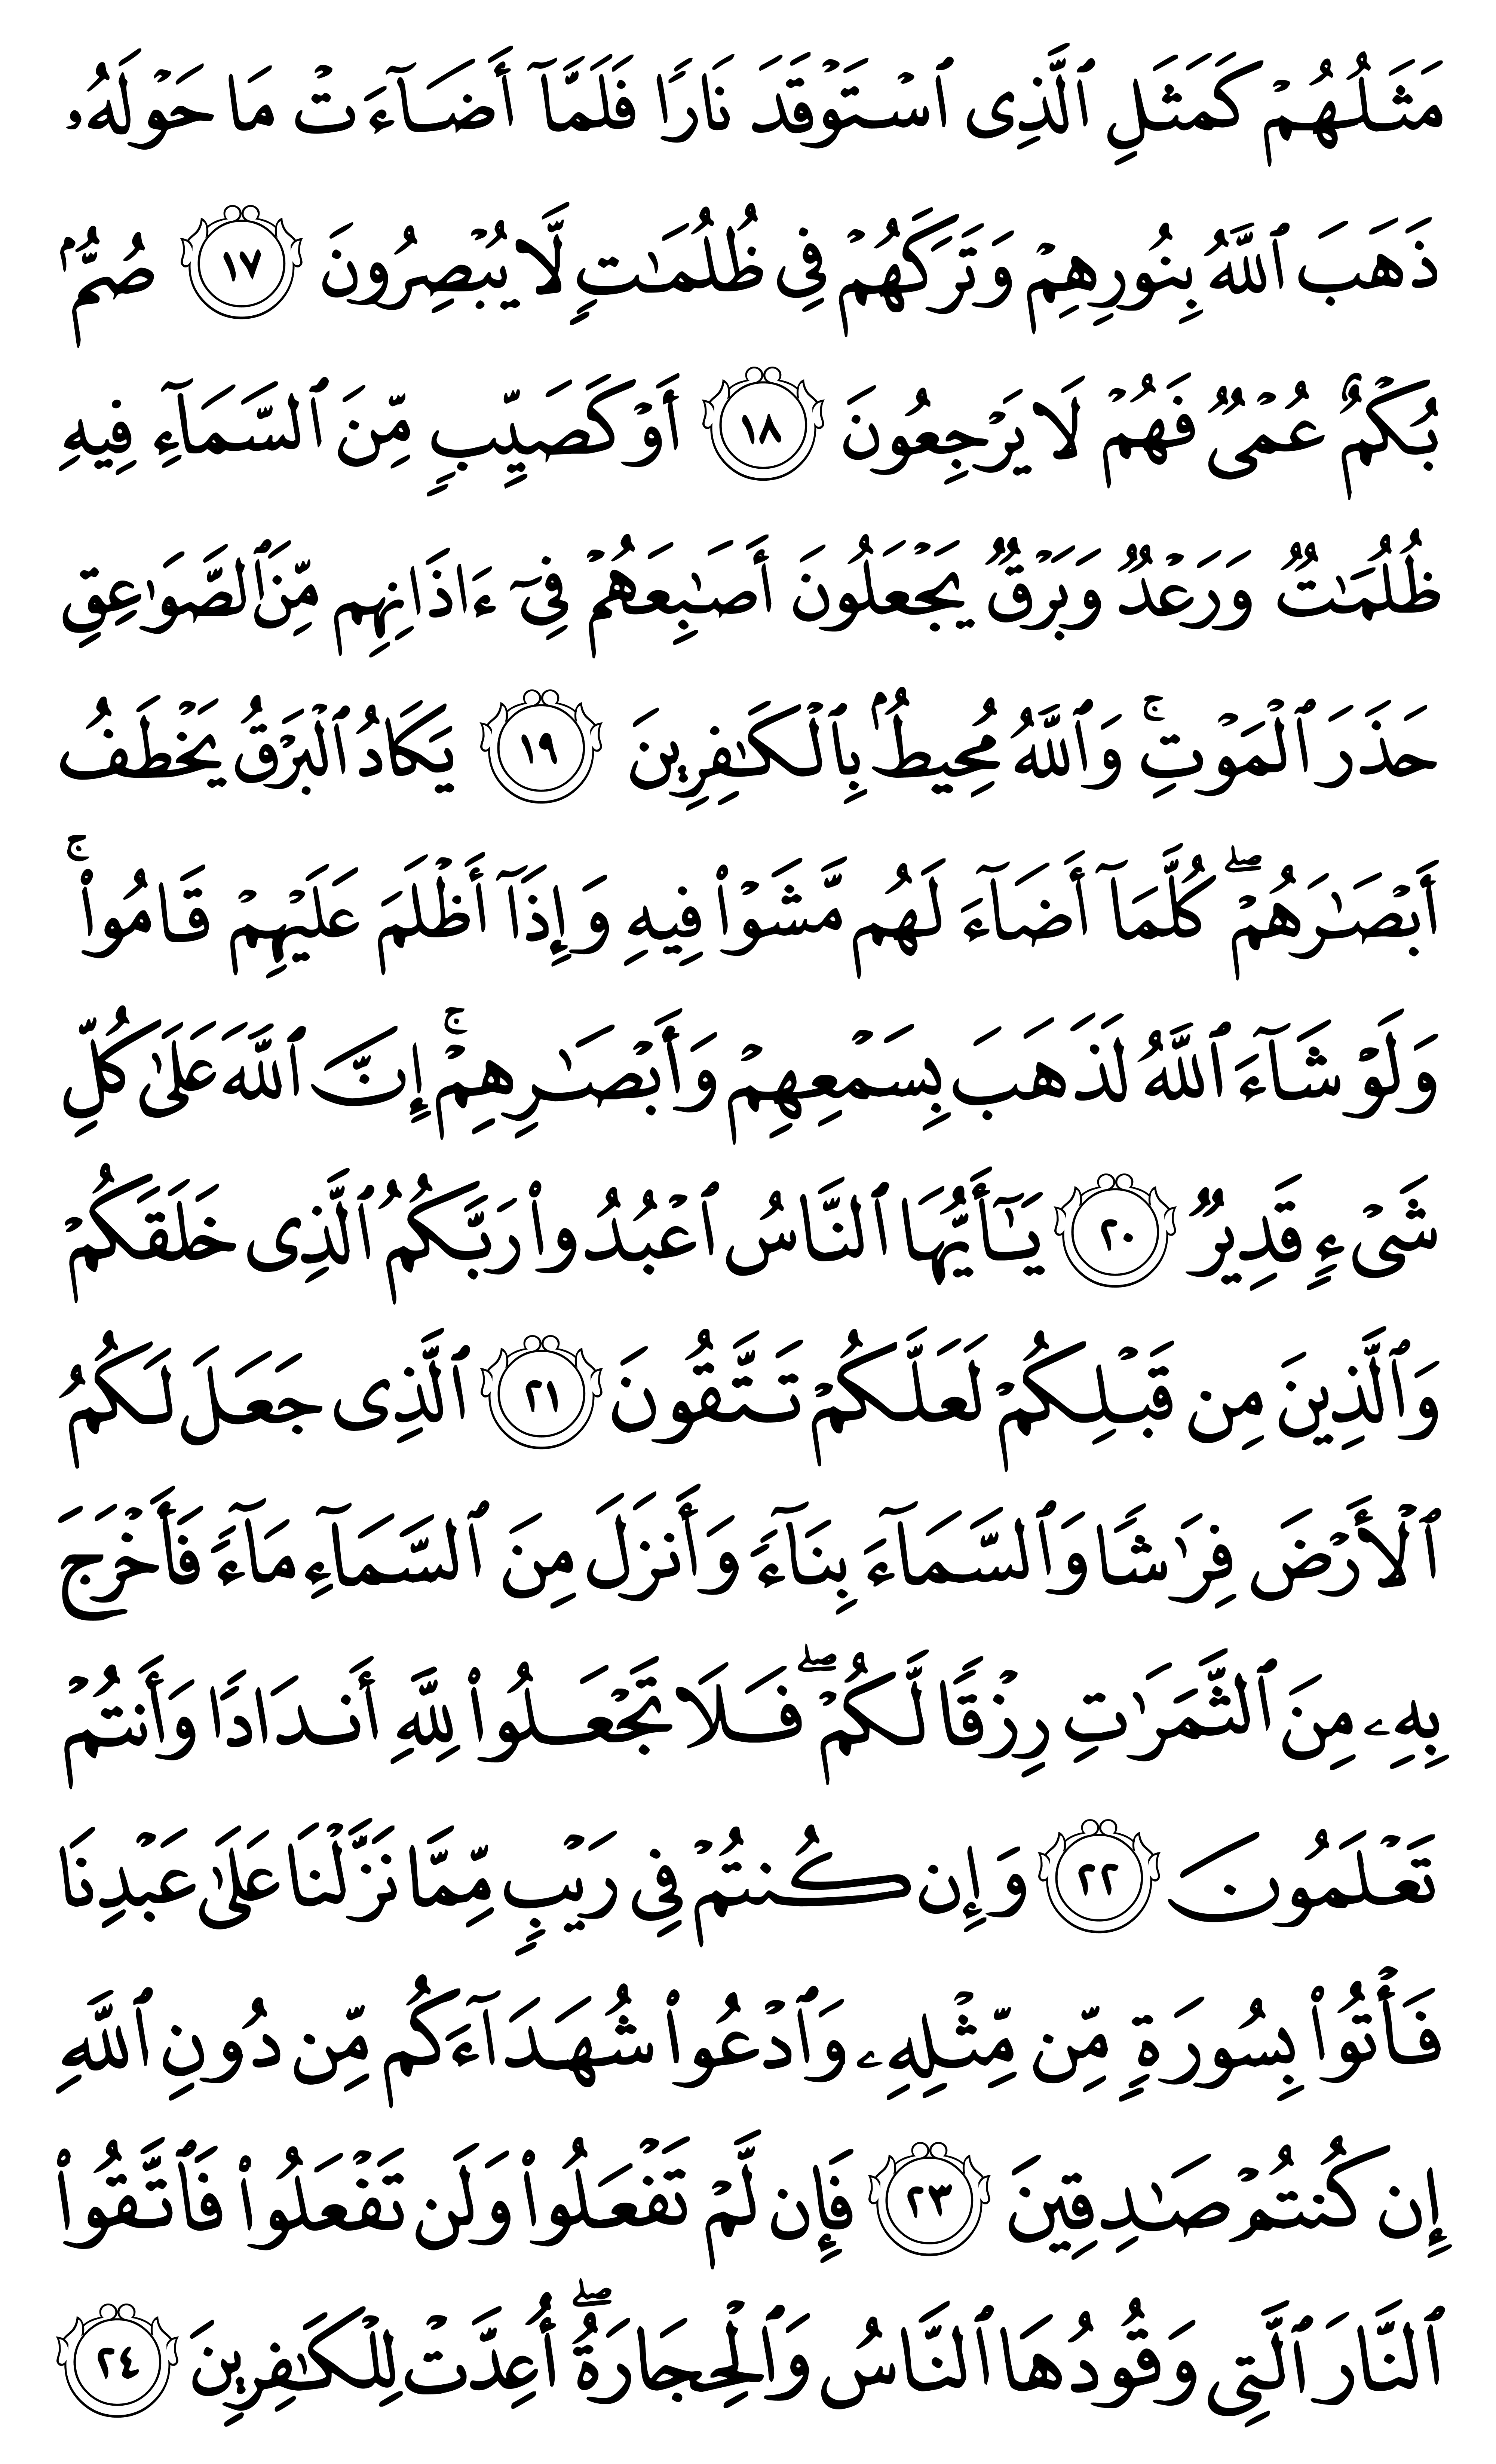
\includegraphics[width=\textwidth,height=\textheight,keepaspectratio]{images/004.png}
\end{center}

\end{document}